\documentclass{letter}
\usepackage{hyperref}
\usepackage{color}
\usepackage{graphicx}

\newcommand\newnotecommand[3]{%
  \newcommand#1[1]{{\color{#3}{\color{#3}#2:} ##1}}}
\newnotecommand\authorreply{Author Reply}{red}


\signature{The authors of NEUCOM-D-14-02709}
\address{Tampere University of Technology\\University of Southern Denmark}
\begin{document}

\begin{letter}{Special Issue Editor and Anonymous Reviewers\\
Submission NEUCOM-D-14-02709\\
Neurocomputing}

\opening{Dear Sir or Madam:}

We thank editor and anonymous reviewers for their valuable comments.
We have revised the manuscript and in
the following we briefly reply to the reviewers' comments.

{\em Reviewer \#1:}
Manuscript Number NEUCOM-D-14-02709 compares some of the existing local feature
detectors and descriptors for object class matching.  This is an interesting,
well-written and experimentally intensive investigation. 

Comments:

1)	Besides these set of descriptors, it would be interesting to include both LIOP and RFGd.

\authorreply{Of the two we found an implementation for the LIOP descriptor and evaluated it with our framework (see the figure below). The results were worse than those selected for our comparison and therefore not included to the revised manuscript for clarity (many other descriptors were evaluated as well, but only the best selected). However, a reference to the LIOP was added and it is included to our public code.}

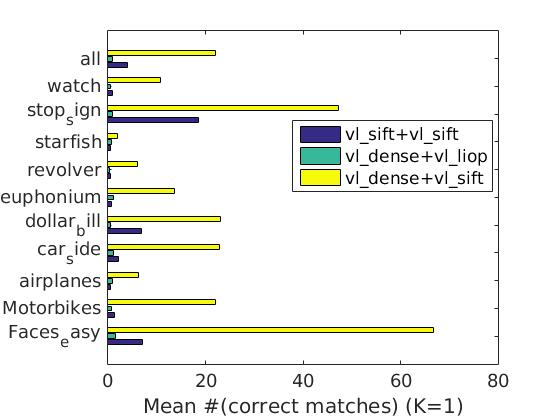
\includegraphics[width=0.5\linewidth]{resources/liop.jpg}

2)	The standard metric for quantitative evaluation of descriptor matching is
the recall vs 1-precision plot. This is lacking in this manuscript, which makes it
a little difficult for readers to compare and contrast the experimental findings
for each performance evaluation against existing performance evaluation works.

\authorreply{This was considered during the course of our work, but since our case is a bit different from other works that deal with the wide baseline setting (e.g., Mikolajczyk and Schmid, PAMI 2005) where image pairs are tested one by one we decided to report the average number of matches that is more compact and intuitive for a large set of image pairs containing category instaces. The average numbers were also reported in the original work of Mikolajczyk and Schmid, PAMI 2005 (Table 2).}

3)	A section reporting the computational processing time would also be useful,
especially when dense sampling can be pretty time-consuming.

\authorreply{The computation times are now added to the results table in Figure 5.}

4)	Perhaps the authors can consider the effects of illumination, scale and
defocusing for the mix of feature detectors and descriptors.

\authorreply{We agree that this would be another interesting research direction, but
we particularly decided to focus on robustness to appearance variation between class examples which has not been studied in similar extent before. Moreover, the mentioned imaging distortions have been partially investigated in the wide baseline matching setting (e.g. Mikolajczyk et al. PAMI 2005 and IJCV 2005)}

{\em Reviewer \#2:}
 The paper presents a framework of comparing feature detectors and descriptors
on object class matching. It also evaluate the common widely feature detector
and descriptors on this framework. Some interesting observations are concluded.
But one shortcoming is the paper miss the efficiency comparison of the
detectors and features. For example, in their second finding, densing sampling
outperforms interest point detectors. In fact, the efficient of densing
sampling may be not better than the later one. It would be useful if they could
give the efficiency comparison.

\authorreply{Computation times are now added to the results table in Figure 5. We agree that dense sampling is less efficient, but since it does not need the detector part it is actually surprisingly fast if properly implemented.}

In line 125, the adjustment of meta-parameters makes the Hessian-affine do
worst. Please provide the results between them. Further, it would be useful
to explain why it will become worst.

\authorreply{The original values are now added for comparison.}

In line 165, the 1) and 2) is not clear. What is anything for the combination?

\authorreply{This was clarified ``With the default parameters the first two detector-descriptor pairs using the Mikolajczyk's implementation...''}

In line 205, as they said, the best discriminative methods perform well on
detection rather than classification. But what is the best discriminative
methods here? Additionally, the paper didn't analyze the reason why it
badly work in classification. It would be better if they could clarify them.

\authorreply{Here we wanted to point out that local region detectors, in general, perform rather fine, but the evaluated local region descriptors were not able to match the corresponding areas between images. This is clarified in the revised manuscript.}

The paper now presents a figure (Figure 8) with matching number bars. Fonts
are very small, the color bar is very dense. No statistical tests with
significance levels are reported. Are the readers expected to eye ball the
data for significance?

\authorreply{The figure content is now vertical instead of horizontal making plots larger. Moreover, we emphasize that the differences between the methods are not as interesting as the finding that the number of matches clearly increases with the increased number of nearest neighbors (saturating between 5 to 10).}

Figure 5 (a), what is the 'K' in X-axis? What kind of classifier is used in
object matching? What is the correct matching for each category when the
different overlap threshold is used?

\authorreply{$K$ actually refers to the more advanced experiment in Sec. 4.2 and clarification was added to the figure caption.}

\closing{Yours Faithfully,}

\ps

%P.S. You can find the full text of GFDL license at
%\url{http://www.gnu.org/copyleft/fdl.html}.

%\encl{Turnitin overall score page}

\end{letter}
\end{document}
